%%
%% This is file `mcmthesis-demo.tex',
%% generated with the docstrip utility.
%%
%% The original source files were:
%%
%% mcmthesis.dtx  (with options: `demo')
%%
%% -----------------------------------
%%
%% This is a generated file.
%%
%% Copyright (C)
%%     2010 -- 2015 by Zhaoli
%%     2014 -- 2016 by Liam 
%%     2017 -- 2019 by Xuehan
%%
%% This work may be distributed and/or modified under the
%% conditions of the LaTeX Project Public License, either version 1.3
%% of this license or (at your option) any later version.
%%
%% This work has the LPPL maintenance status `maintained'.
%%
%% The Current Maintainer of this work is Xuehan.
%%
\documentclass{mcmthesis}
\mcmsetup{CTeX = false,   % 使用 CTeX 套装时,设置为 true
        tcn = 55280, problem = A,
        sheet = true, titleinsheet = true, keywordsinsheet = true,
        titlepage = true}
\usepackage{palatino}
\usepackage{mwe}
\usepackage{graphicx}
\usepackage{subcaption}
\usepackage{float}
\usepackage{multirow}
\usepackage{indentfirst}
\usepackage{gensymb}
\usepackage[ruled,lined,commentsnumbered]{algorithm2e}
\usepackage{diagbox}



\usepackage{geometry}
\geometry{left=2cm,right=2cm,top=2cm,bottom=2cm} %%页边距,若对左右边距进行修改,请保证左右边距一样,并且将mcmthesis.cls第81行对应的margin参数设置为相同数值
\begin{document}
\linespread{0.6} %%行间距
\setlength{\parskip}{0.5\baselineskip} %%段间距
\title{ti}

\date{\today}
\begin{abstract}
 		This is the \textbf{Abstract Part}

	\begin{keywords}
	keywords1,keywords2,keywords3
	\end{keywords}
\end{abstract}

\maketitle

\tableofcontents
\newpage

\section{Example For Section}


\subsection{Example For SubSection}


\subsubsection{Example For SubSubSection }

Example for Fig.~\ref{fig:eg1}.

\begin{figure}[H]
	\centering
	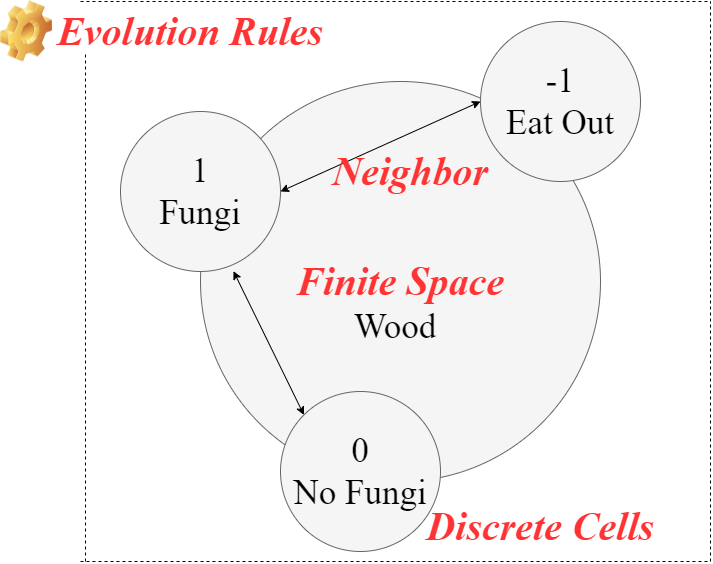
\includegraphics[width = 0.7\textwidth]{CA.png} 
	\caption{e.g.}
	\label{fig:eg1}
\end{figure}

Example for Tab.~\ref{tbl:eg1}.

\begin{table}[H]
	\centering
	\caption{e.g}
	\begin{tabular}{|c|c|c|}
	\toprule
	  & Symbol &Definition\\
	\midrule
	1 & 2 & 3\\	
	1 & 2 & 3\\
	1 & 2 & 3\\
	1 & 2 & 3\\
	1 & 2 & 3\\
	\bottomrule
	\end{tabular}
	\label{tbl:eg1}
\end{table}


\begin{algorithm}[H]
	\SetAlgoLined
	\KwIn{$\lambda_0$, $\lambda_{max}$, $\omega$, $x_{0,ini}$, $\delta$, $n_{max}$,}
	\KwResult{$\Sigma P$, $f_{t1}$, $f_{t2}$, $score$}
	\While{there are other combinations of $(\lambda, n, x_0)$}{
		the distribution of the force $f(x)$ \\
		the position of the rod $g(i, n, L, \lambda)$ \\
		get the force on each rod $f_i(i, n, F, X, x0)$ \\
		calculate tention $[f_{i,1}, f_{i,2}] = T_i([x0, y0], [x1, y1], [x2, y2], f_i)$ \\
		next $(\lambda, n, x_0)$ \\
	}
	Data normalization for $(f_{i, 1}, f_{i, 2}, (\Sigma P)_i)$ \\
	Score $= \frac{\omega}{2}(f_{i, 1} + f_{i, 2}) + (1 - \omega)(\Sigma P)_i$
	\caption{Cellular Automata Simulation of F}
\end{algorithm}

\par Cellular automata is a model that defines \textbf{a finite space} and a series of \textbf{discrete cells}. These cells will automatically evolve according to the different states of their eight \textbf{neighbors} and follow certain \textbf{evolution rules}. It is a dynamic and discrete system which can simulate the growth, decomposition and competition of various fungi on the wood very well. Fig.(\ref{f1ForCA}) shows a brief sketch of cellular automata model.

\begin{figure}[H] 
	\centering 
	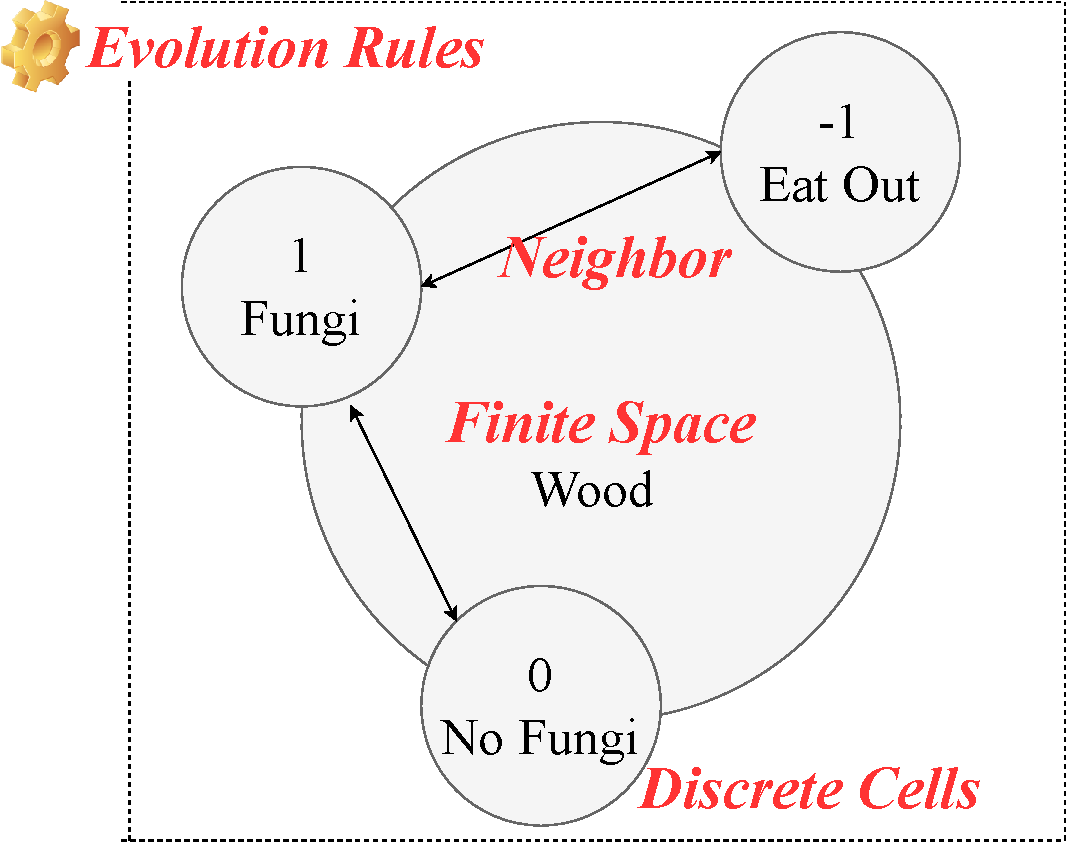
\includegraphics[height=7cm]{./picture/CA.pdf}
	\caption{Cellular automata model}
	\label{f1ForCA}
\end{figure}

\par Fig.(\ref{AS}) is the \textbf{evolution rules} for the fungi cell. In the whole process, the growth speed of the cell follows the modified extension rate which is shown on Eqn.\eqref{???}, the winning probability is defined by Elo rating system which is shown on Eqn.\eqref{???} and the decomposition rate is calculated by Eqn.\eqref{???}.
\begin{figure}[H] 
	\centering 
	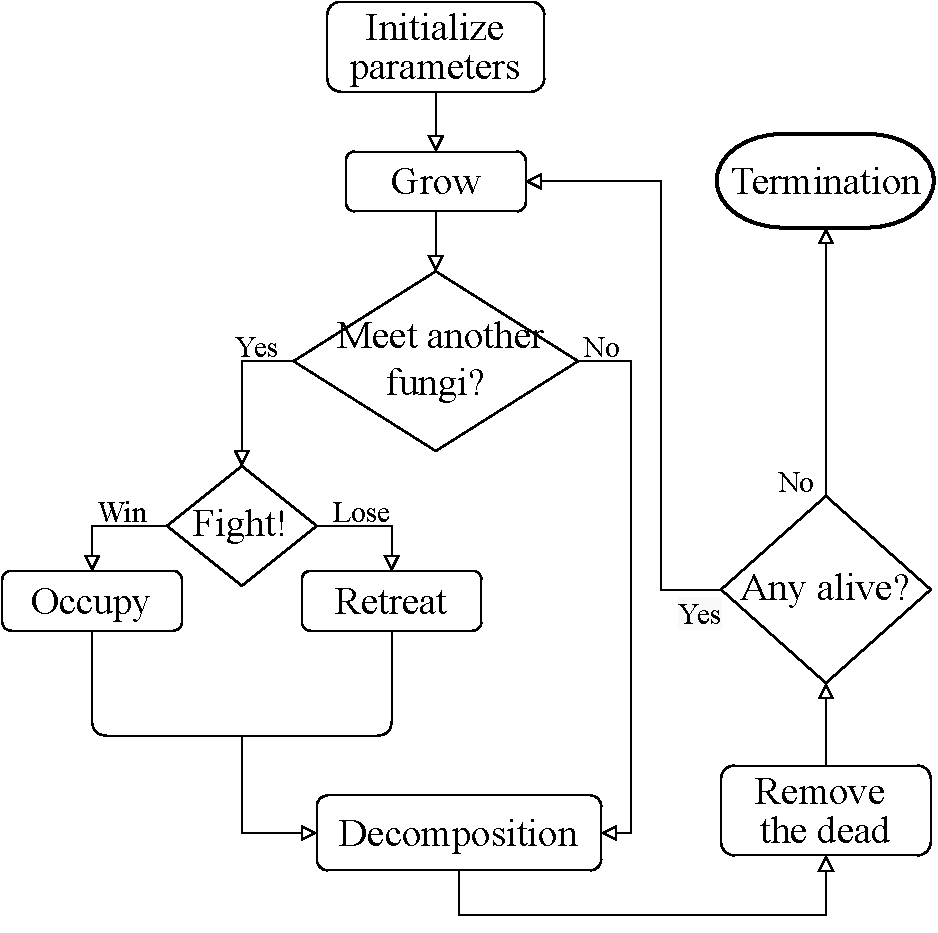
\includegraphics[height=10cm]{./picture/liucheng.pdf}
	\caption{Algorithm schematic}
	\label{AS}
\end{figure}
\par 

\begin{table}[H]
	\centering
	\caption{Notations}
	\begin{tabular}{c|c}
	\hline
	Symbol & Definition \\
	\hline
	$L$ & Beam Length\\
	$E$ &  Modulus of Elasticity of the Beam\\
	$I_B$ & Second Moment of Inertia for the cross section of the beam\\
	$h_0$ & The hight difference between the beam and the top\\
	$\lambda$ & Quadratic equation constant\\
	$\lambda$ & Quadratic equation constant\\
	$W$ & Weight of the trailer\\
	$n$ & Number of the rod\\
	$P_b$ & Unit price of the beam(1m)\\
	$P_r$ & Unit price of the rod(1m)\\
	$P_c$ & Unit price of the cable(1m) \\
	\hline
	\end{tabular}
\end{table}


\begin{figure}[H] 
	\centering 
	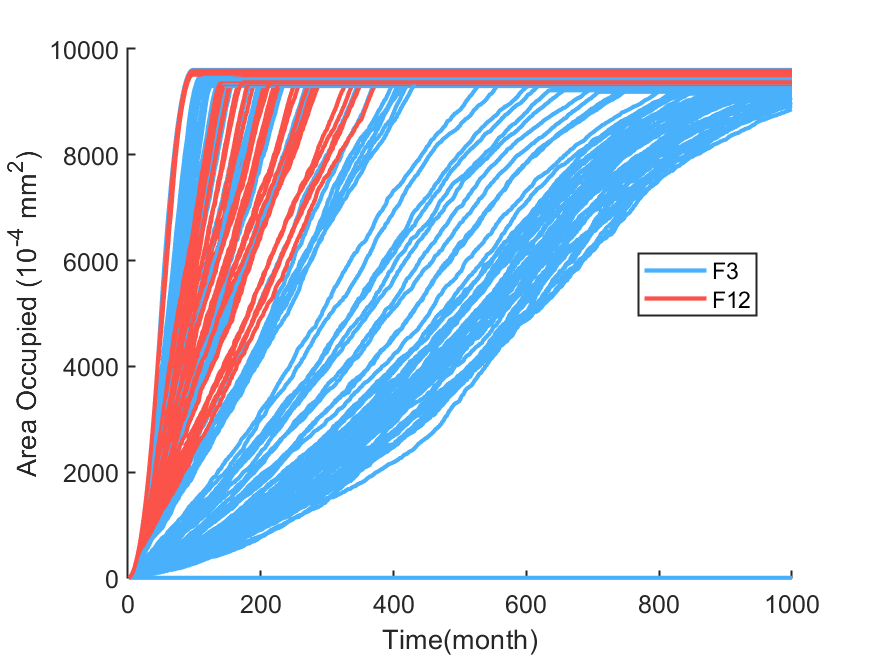
\includegraphics[height=10cm]{./picture/3vs12.eps}
	\caption{Algorithm schematic}
\end{figure}
\par 
\begin{figure}[H] 
	\centering 
	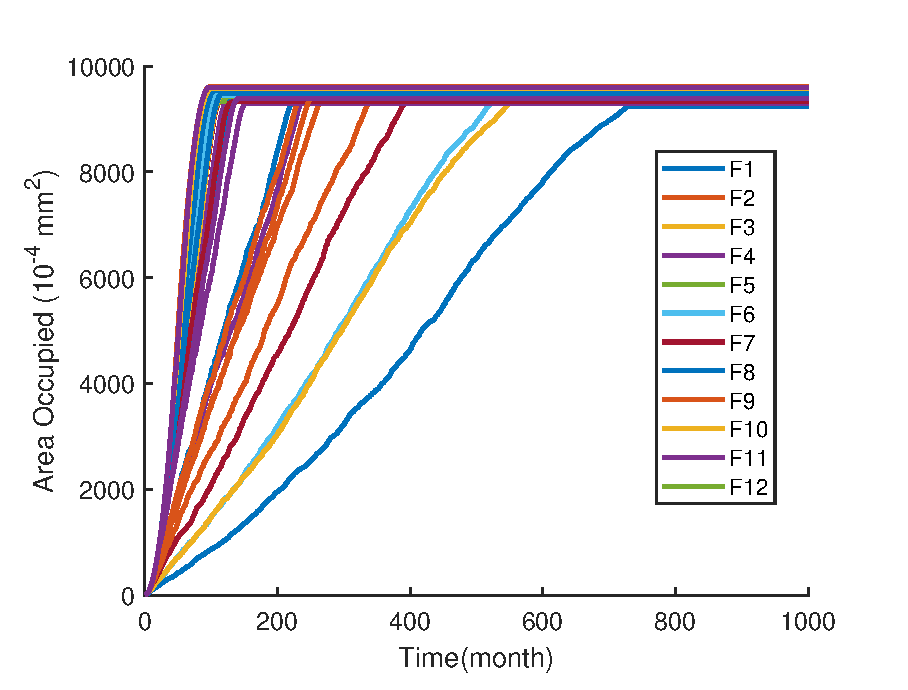
\includegraphics[height=10cm]{./picture/12for5.eps}
	\caption{Algorithm schematic}
\end{figure}
\par 
\begin{figure}[H] 
	\centering 
	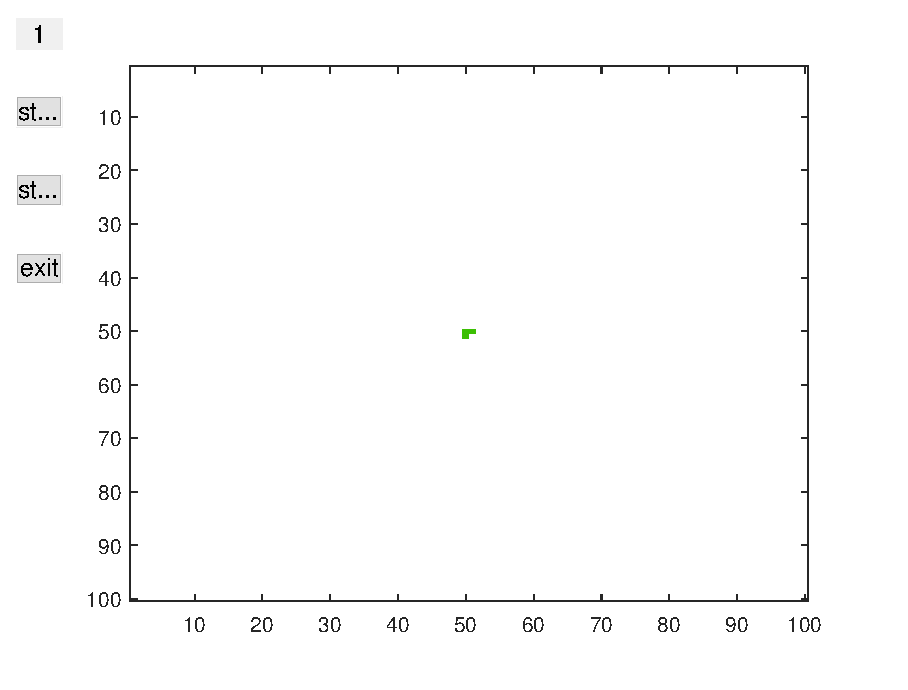
\includegraphics[height=10cm]{./picture/suppose0.eps}
	\caption{Algorithm schematic}
	\label{AS}
\end{figure}
\par 
\begin{figure}[H] 
	\centering 
	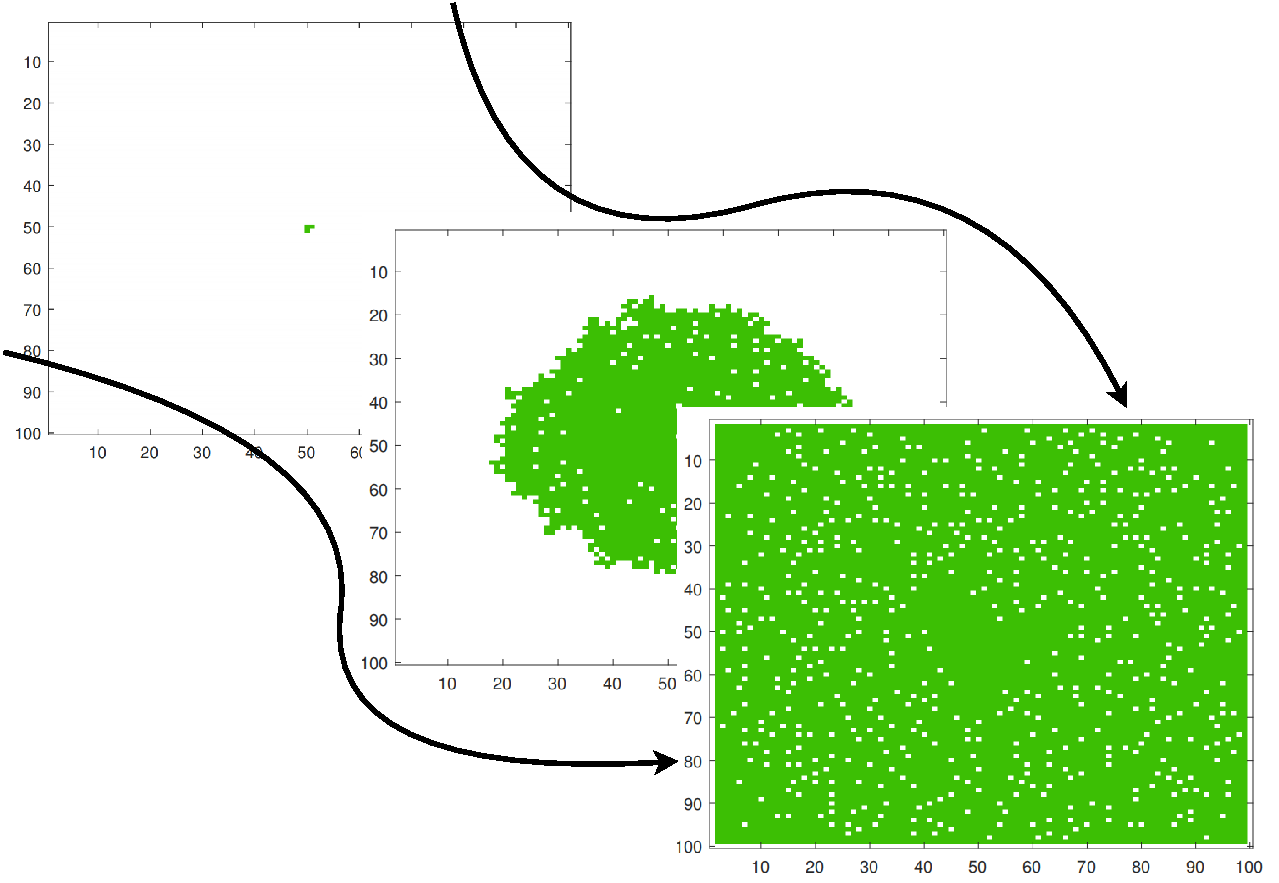
\includegraphics[height=10cm]{./picture/SJflow.pdf}
	\caption{Algorithm schematic}
\end{figure}




\begin{algorithm}[H]
	\SetAlgoLined
	\KwIn{$\lambda_0$, $\lambda_{max}$, $\omega$, $x_{0,ini}$, $\delta$, $n_{max}$,}
	\KwResult{$\Sigma P$, $f_{t1}$, $f_{t2}$, $score$}
	\While{there are other combinations of $(\lambda, n, x_0)$}{
		the distribution of the force $f(x)$ \\
		the position of the rod $g(i, n, L, \lambda)$ \\
		get the force on each rod $f_i(i, n, F, X, x0)$ \\
		calculate tention $[f_{i,1}, f_{i,2}] = T_i([x0, y0], [x1, y1], [x2, y2], f_i)$ \\
		next $(\lambda, n, x_0)$ \\
	}
	Data normalization for $(f_{i, 1}, f_{i, 2}, (\Sigma P)_i)$ \\
	Score $= \frac{\omega}{2}(f_{i, 1} + f_{i, 2}) + (1 - \omega)(\Sigma P)_i$
	\caption{Optimal Architecture}
\end{algorithm}
\newpage

\par Then the celluar automata model will be used to simulate how a single fungus grow under random and rapid environmental changes. Article ??? claims that the hyphae of fungi that can better adapt to the environment are denser and expand more slowly, so will they have high adaptability in this random environment? We mainly measure the change of the surface area of a fungus on 100[mm] $\times$ 100 [mm] wood blocks. It will expand from the center until covering the whole block. Fig.\eqref{sjsjsj} shows the process and area change curve for 12 different fungi under 5 different random conditions.
\begin{figure}[H]
	\centering
	\begin{subfigure}{0.45\textwidth}
		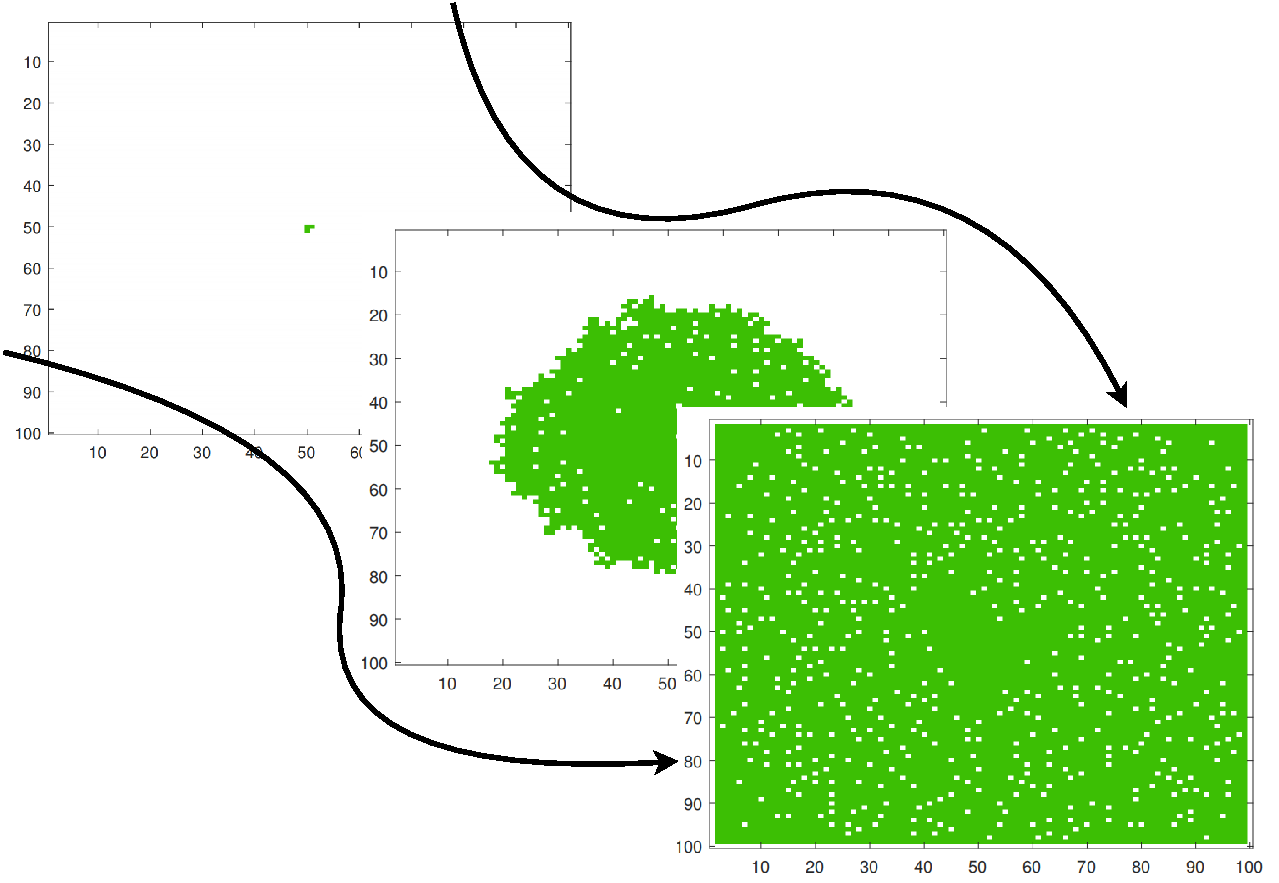
\includegraphics[width=\textwidth]{./picture/SJflow.pdf}
	\end{subfigure}
	\begin{subfigure}{0.45\textwidth}
		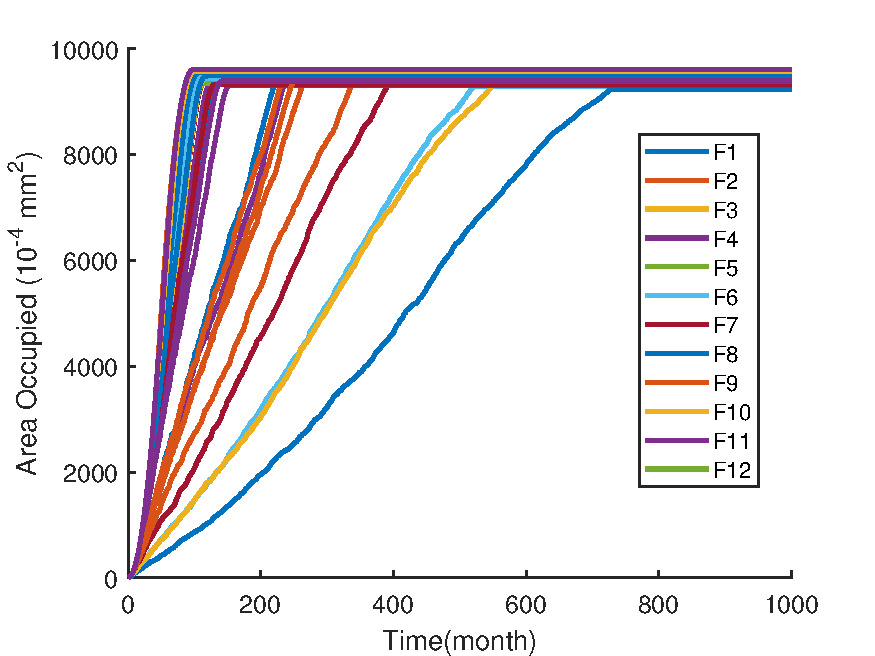
\includegraphics[width=\textwidth]{./picture/12for5.pdf}
	\end{subfigure}
	\caption{Tset process and results for rapid fluctuations in $T$ and $m$.}
	\label{sjsjsj}
\end{figure}
From the Fig.\eqref{sjsjsj}, we can find that some color curve families, such as F3-orange curve family, do not deviate too much from each other and almost grow in the same trend, while some color curve families, such as blue-F8 curve family in, deviate much from each other. This is because fungi like F3 have a higher moisture niche width and temperature niche widt so when they face the fluctuation of the environment, their range of change is smaller which means that they are more \textbf{stable}.
\begin{figure}[H] 
	\centering 
	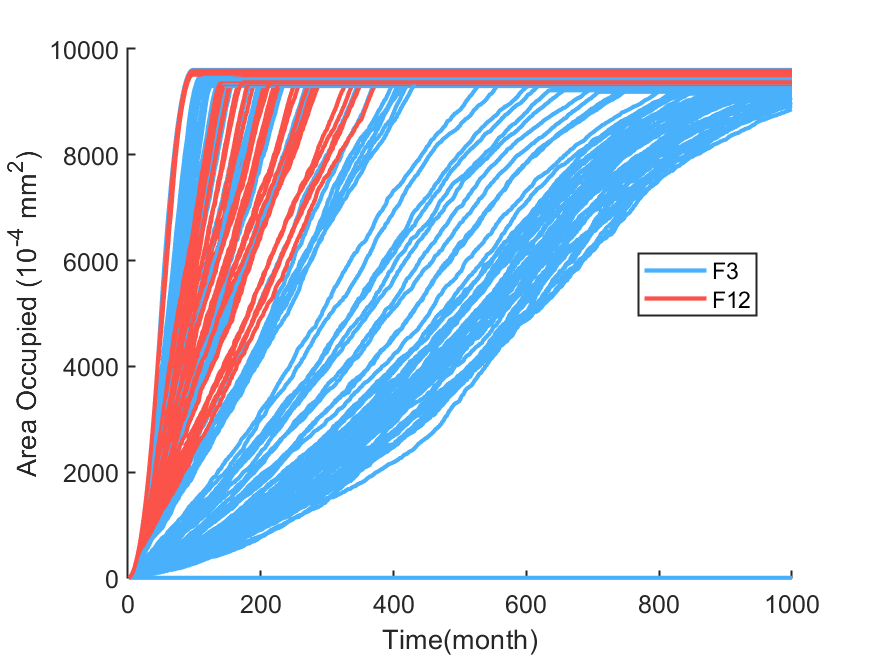
\includegraphics[height=7cm]{./picture/3vs12.pdf}
	\caption{Area change curves of F3 and F12 (50 for each).}
	\label{spspsp}
\end{figure}
\par Also, this kind of stability will also affect the speed of expension. For example, the expension speed of F12 fungi is 0.77 mm/day while the expension speed of F3 is greater than F12 which is 1.09 mm/day. However on Fig.\eqref{spspsp}, we repeat the simulation 50 times for F3 and F12 and can conclude that the average expantion speed of F12 is far more than F3 which means that those kind of fungi that are more stable will also have \textbf{advantage on expansion speed} when facing great change on emvironment. 

\bibliographystyle{IEEEtran}
\bibliography{newrefs}

\newpage


\section{Importance of Biodiversity}

\par As introduced in Section 1, the breakdown of ground litter is an important process in ecological cycles. Therefore, the efficiency of decomposition is one of the determinants of the efficiency of ecosystems. In order to study the importance of species diversity of fungi, we are going to test whether the diversity of species will improve the efficiency of decomposition and adaptation to variable environments.
\subsection{Fungi Combination Selection}
\par First of all, according to the results of the previous models, we can get the following rules on the selection of fungi.
\begin{itemize}
	\item According to the analysis of XXXXXX(task 1 name) and xxxxx(task Boston name), we need to choose species that can coexist peacefully on long-term trends to ensure the \textbf{stability of biodiversity}.
	\item From xxxxx(fluctuation model name), we can know that the decomposition rate of bacteria is sensitive to environmental changes, so the \textbf{adaptability and viability} of fungi are considered prior to the expansion rate of bacteria. Moreover, when different fungi are combined, the temperature and moisture niche width that the whole system have should be maximized.
	\item When the above two conditions are satisfied as much as possible, we should choose the combination of fungi that expand as fast as possible, because they show great advantages when we do not consider the environmental impact in our initial model.	
\end{itemize}
\par So that according to the previous rules, we can set 5 groups with the same initial numbers of fungi and the same initial positions. 
\begin{table}[H]
	\centering
	\caption{Groups Setting}
	\begin{tabular}{|c|c|c|c|c|c|}
		\hline
		&Group 1 & Group 2 & Group 3 & Group4& Group5\\
		\hline 
		Fungi choose&F3 $\times$ 4 & F9 $\times$ 4 & F3 $\times$ 2 \& F5 $\times$ 2 &  F11 $\times$ 2 \& F12 $\times$ 2 & F7, F8, F11, F12\\
		\hline
		Moisture width &1.32&1.57&1.35&5.17&5.17 \\
		\hline
		Temperature width &15.8&18.6&25.0&28.5&29.1 \\
		\hline
	\end{tabular}
\end{table}

\subsection{Results}
\par In the simulation of this section, we fixed the trend of temperature and moisture to be similar to that of semi-arid area and use cellular automata model to run for 1000 days. The following Fig.\eqref{SYHD} shows theremaining wood thickness for the five different groups of fungi.
\begin{figure}[H]
	\centering
	\begin{subfigure}{0.3\textwidth}
		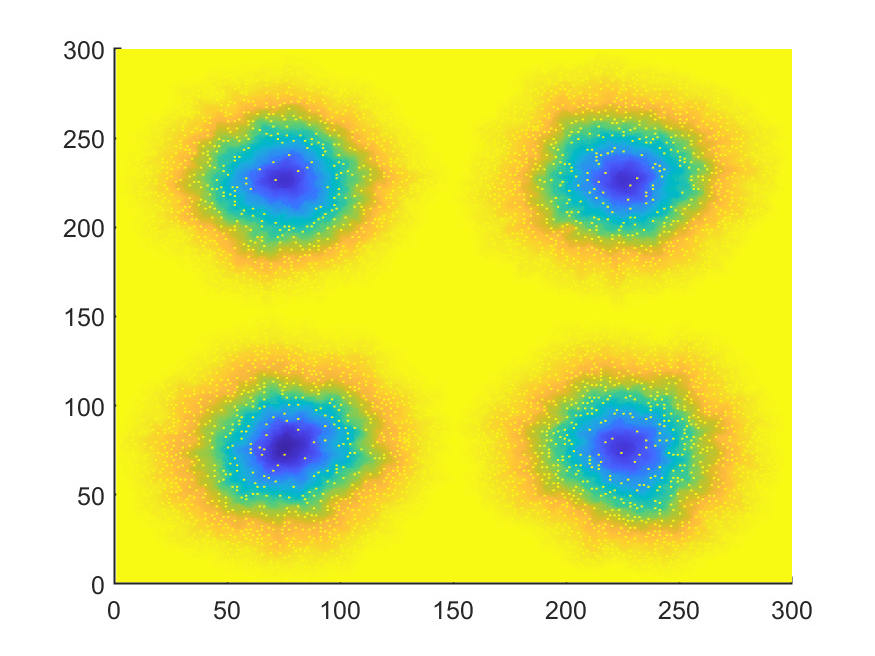
\includegraphics[width=\textwidth]{./T5Figure/K1N1/K1N1L.pdf}
		\caption{F3}
	\end{subfigure}
	\begin{subfigure}{0.3\textwidth}
		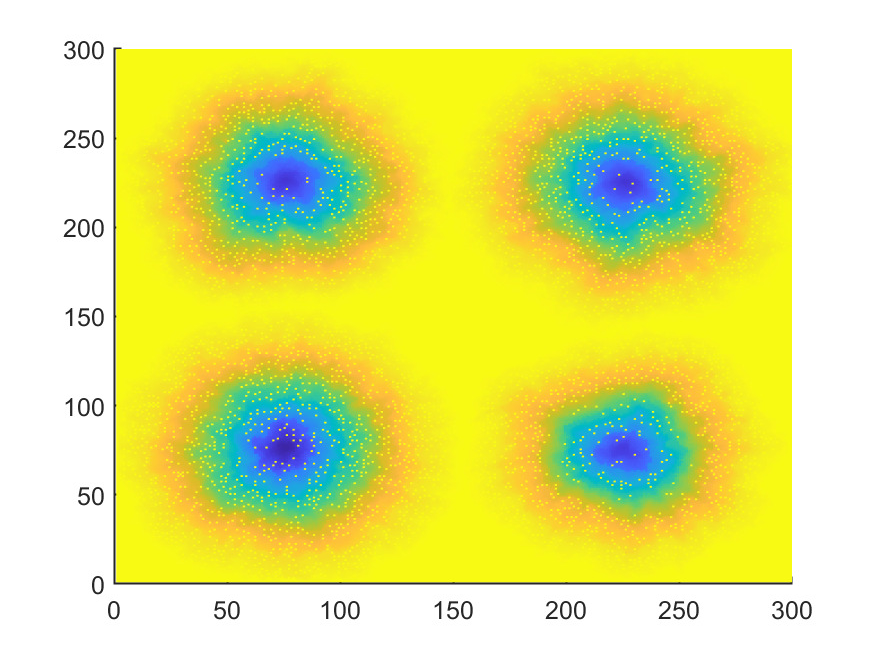
\includegraphics[width=\textwidth]{./T5Figure/K1N2/K1N2L.pdf}
		\caption{F9}
	\end{subfigure}
	\begin{subfigure}{0.3\textwidth}
		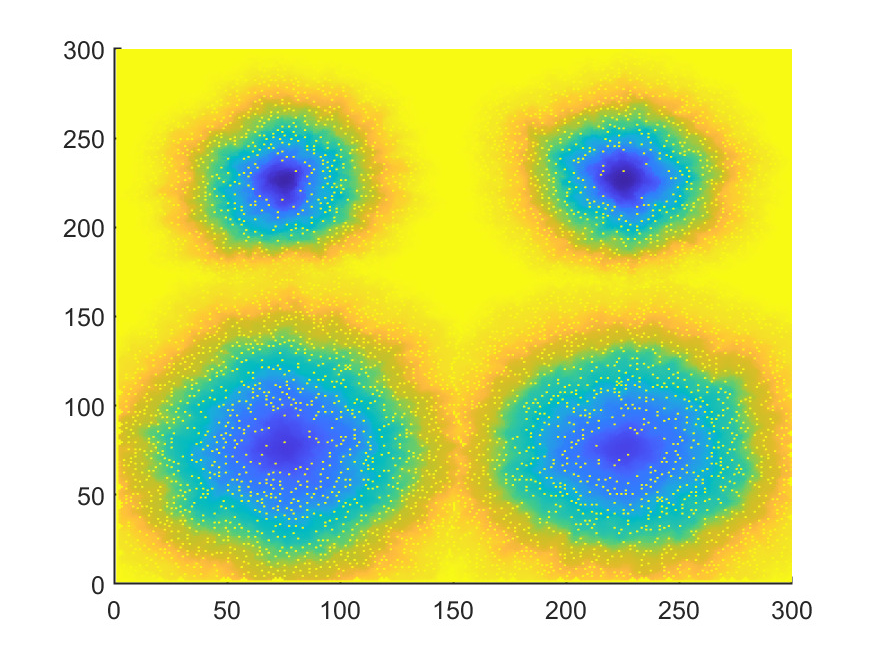
\includegraphics[width=\textwidth]{./T5Figure/K2N1/K2N1L.pdf}
		\caption{F3 F5}
	\end{subfigure}
	\begin{subfigure}{0.3\textwidth}
		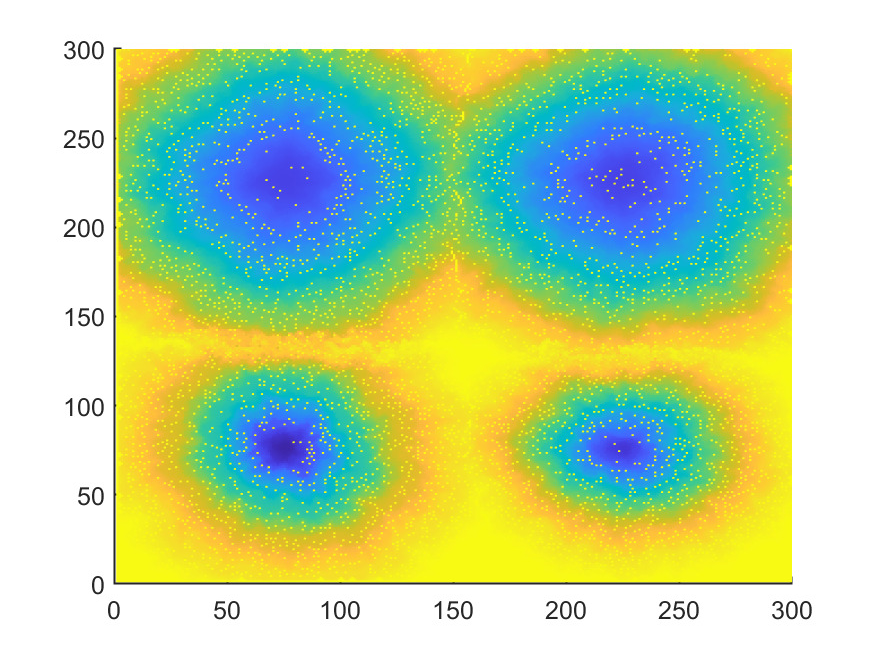
\includegraphics[width=\textwidth]{./T5Figure/K2N2/K2N2L.pdf}
		\caption{F11 F12}
	\end{subfigure}
	\begin{subfigure}{0.3\textwidth}
		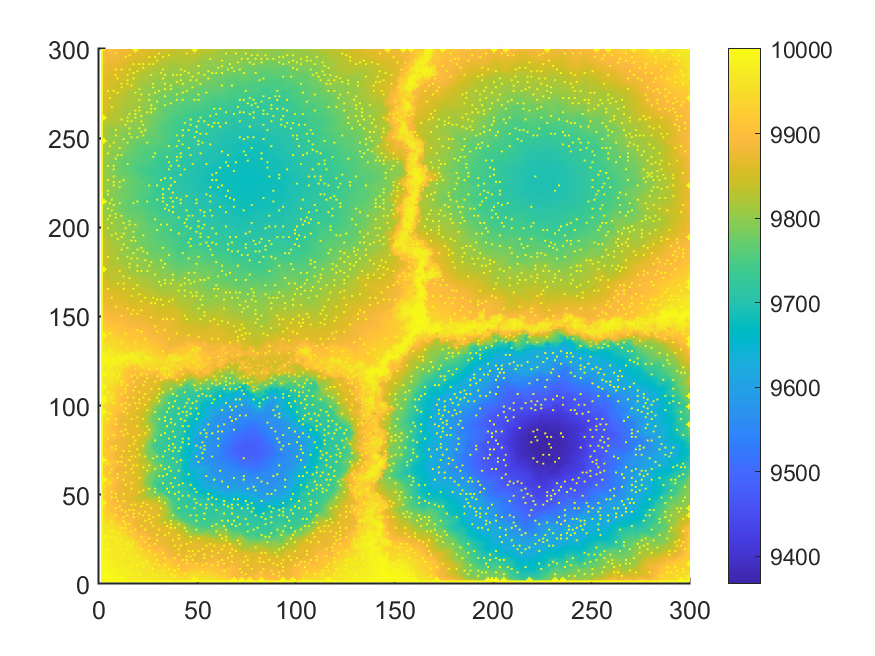
\includegraphics[width=\textwidth]{./T5Figure/K4N1/K4N1L.pdf}
		\caption{F7 F8 F11 F12}
	\end{subfigure}
	\caption{Remaining wood thickness.}
	\label{SYHD}
\end{figure}
\par In order to analyze the process better, we draw the change relationship of the remaining proportion of trees during the process. We set the overall thickness of the wood very large in order to maintain the stability of the system.

\begin{figure}[H] 
	\centering 
	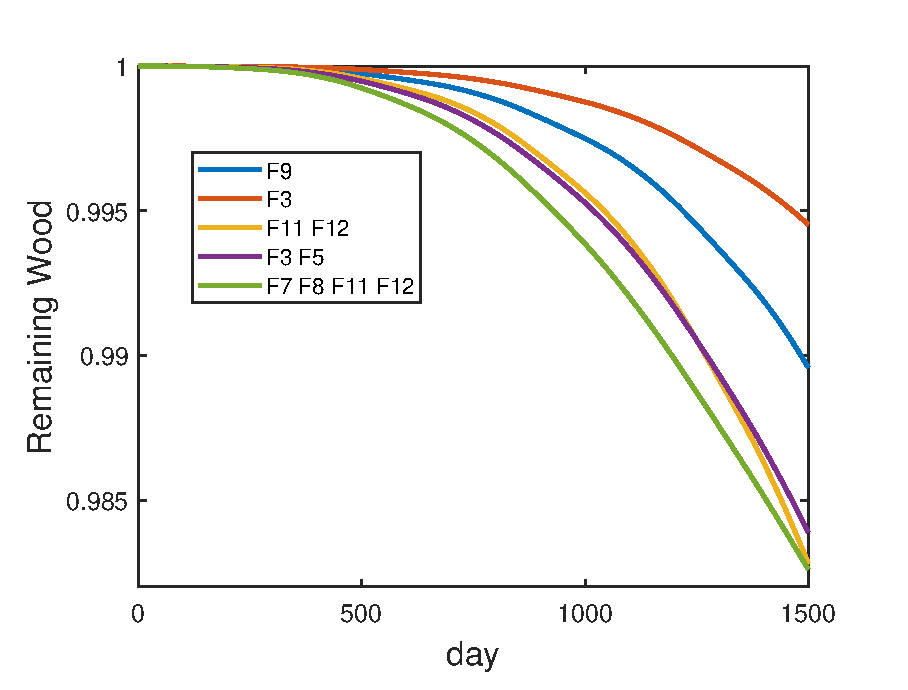
\includegraphics[height=8cm]{./T5Figure/T5overAll.eps}
	\caption{Changes in mass of wood.}
	\label{BHQX}
\end{figure}
\par From Fig.\eqref{BHQX}, we can conclude that when environmental factors are taken into account, biodiversity affects the decomposition rate of fungi. When the total number of fungi and the changing trend of the environment remained unchanged, the decomposition efficiency of the system with four different kind of fungi can reach \textbf{twice} as high as that of a single kind and \textbf{1.25 times} as high as that of two kinds.
\par However, there are preconditions for the conclusion in the previous paragraph, which are \textbf{stability of biodiversity} and \textbf{adaptability and viability} of fungi. Only when these conditions are fully met can we say that the system has \textbf{real biodiversity}.


\begin{figure}[H]
	\centering
	\begin{subfigure}{0.45\textwidth}
		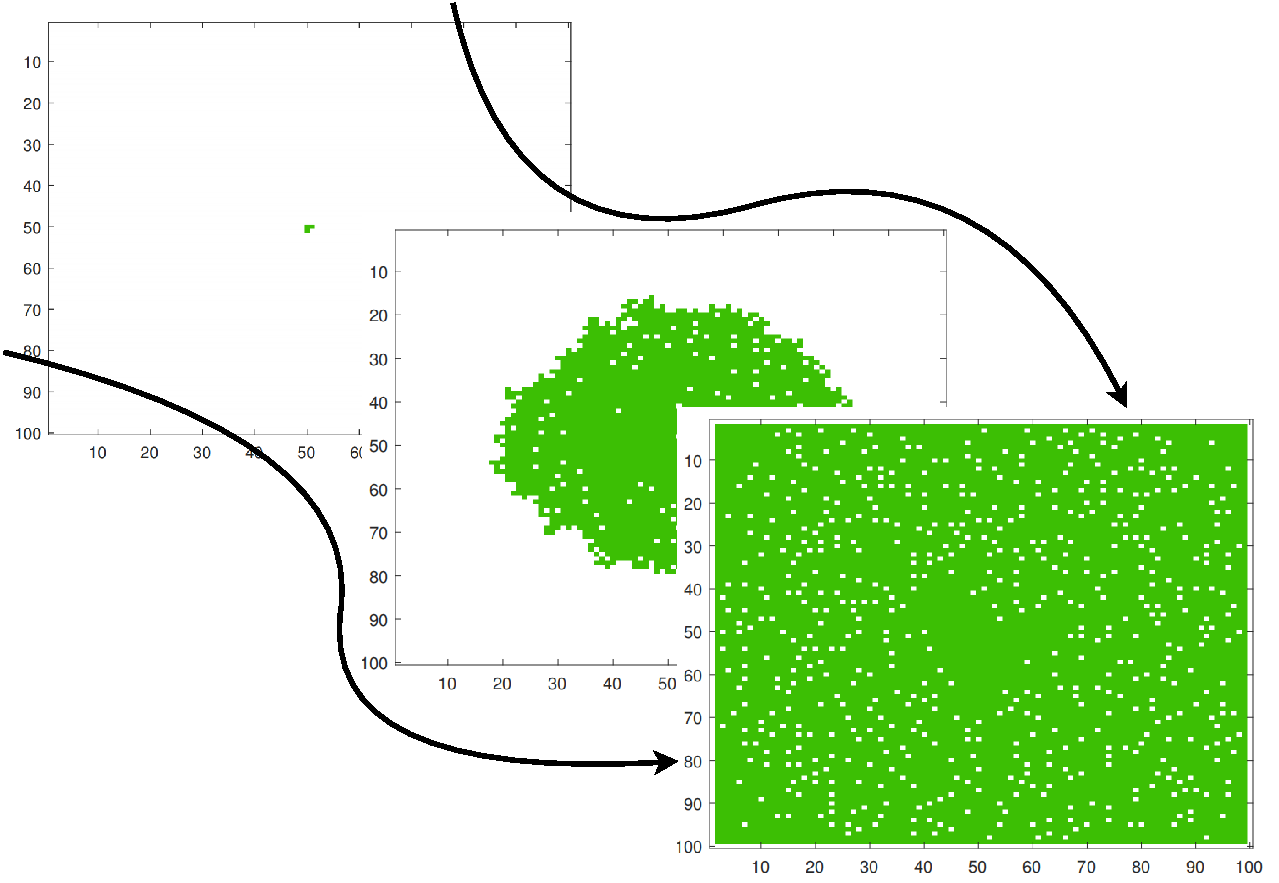
\includegraphics[width=\textwidth]{./picture/SJflow.pdf}
	\end{subfigure}
	\begin{subfigure}{0.45\textwidth}
		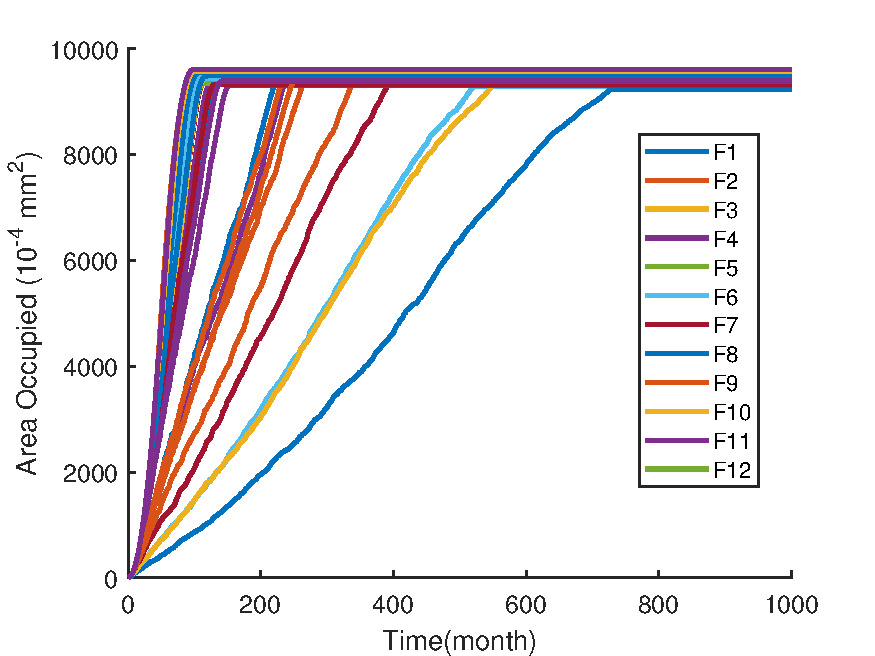
\includegraphics[width=\textwidth]{./picture/12for5.pdf}
	\end{subfigure}
	\caption{Tset process and results for rapid fluctuations in $T$ and $m$.}
	\label{sjsjsj}
\end{figure}


\begin{figure}[H] 
	\centering 
	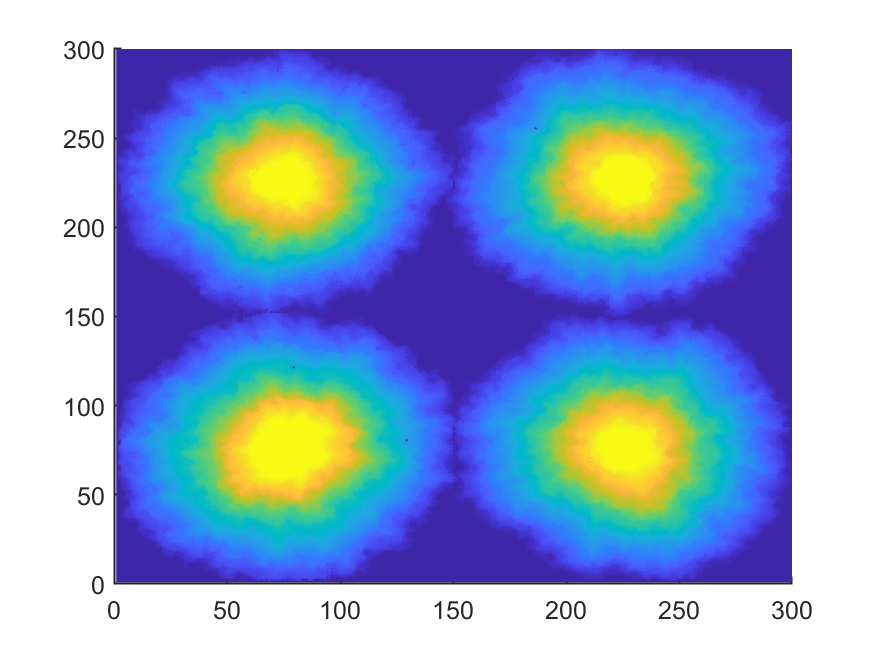
\includegraphics[height=10cm]{./T5Figure/K1N1/K1N1A.pdf}
	\caption{Algorithm schematic}
\end{figure}
\begin{figure}[H] 
	\centering 
	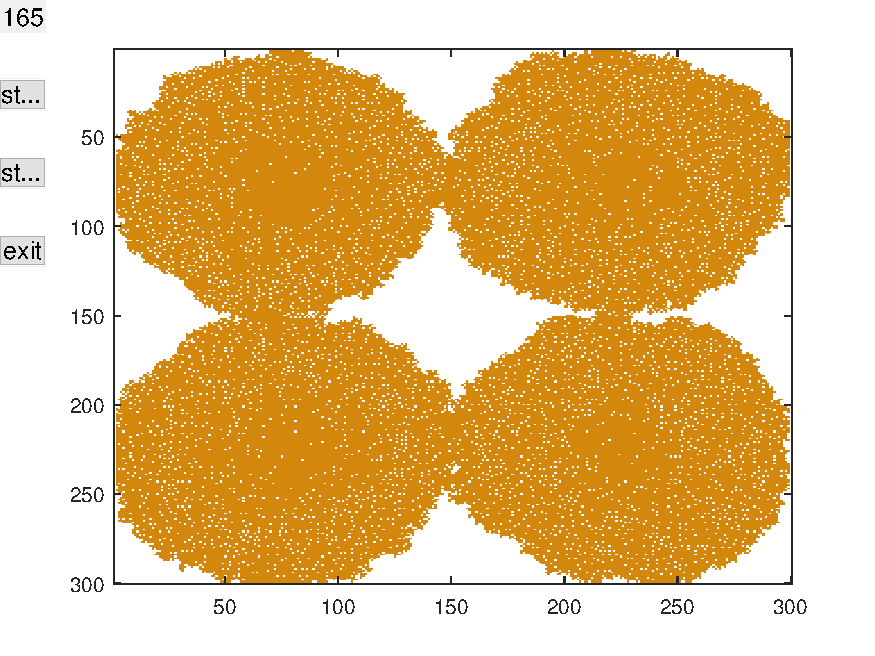
\includegraphics[height=10cm]{./T5Figure/K1N1/K1N1F.pdf}
	\caption{Algorithm schematic}
\end{figure}
\begin{figure}[H] 
	\centering 
	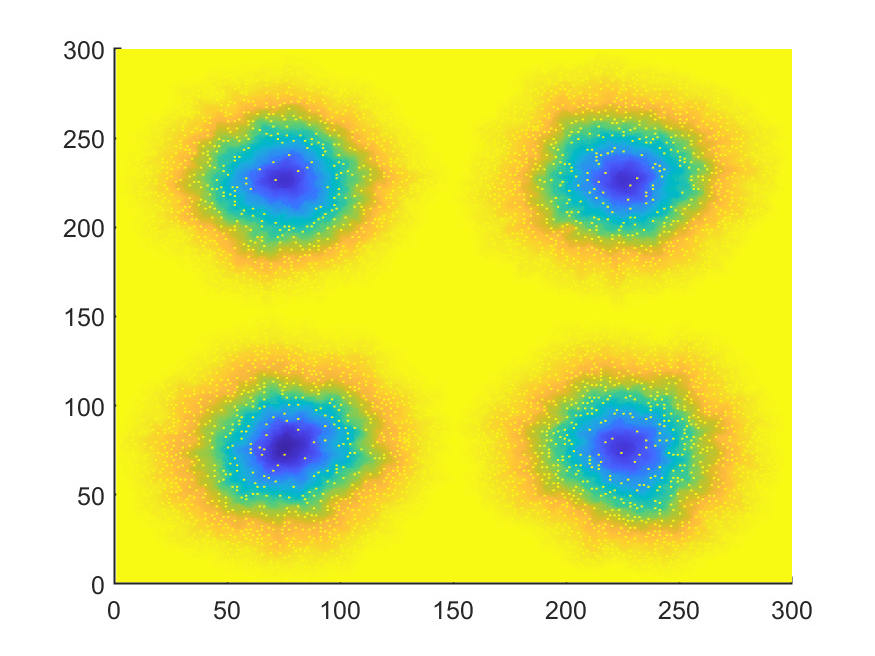
\includegraphics[height=10cm]{./T5Figure/K1N1/K1N1L.pdf}
	\caption{Algorithm schematic}
\end{figure}

\begin{figure}[H] 
	\centering 
	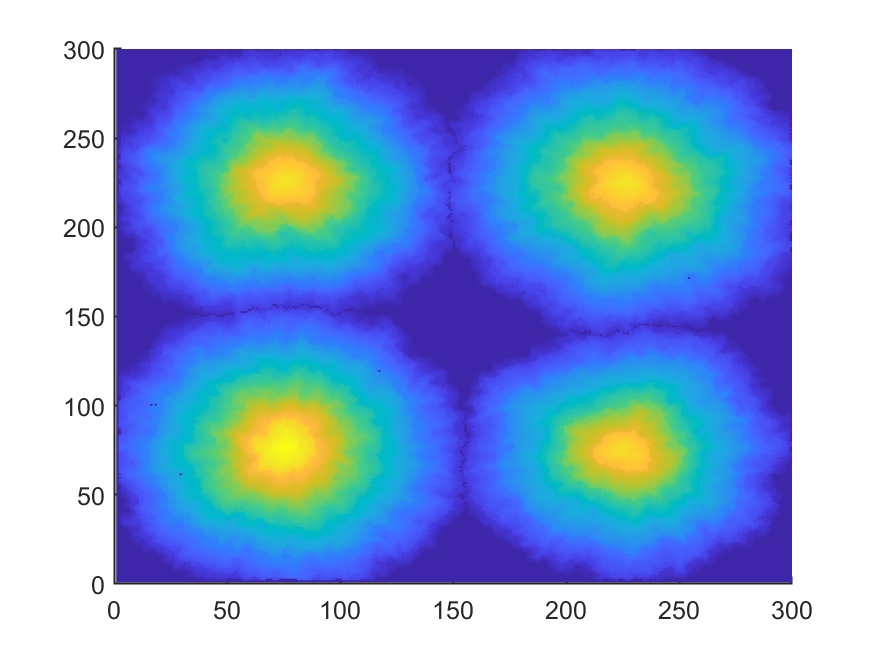
\includegraphics[height=10cm]{./T5Figure/K1N2/K1N2A.pdf}
	\caption{Algorithm schematic}
\end{figure}
\begin{figure}[H] 
	\centering 
	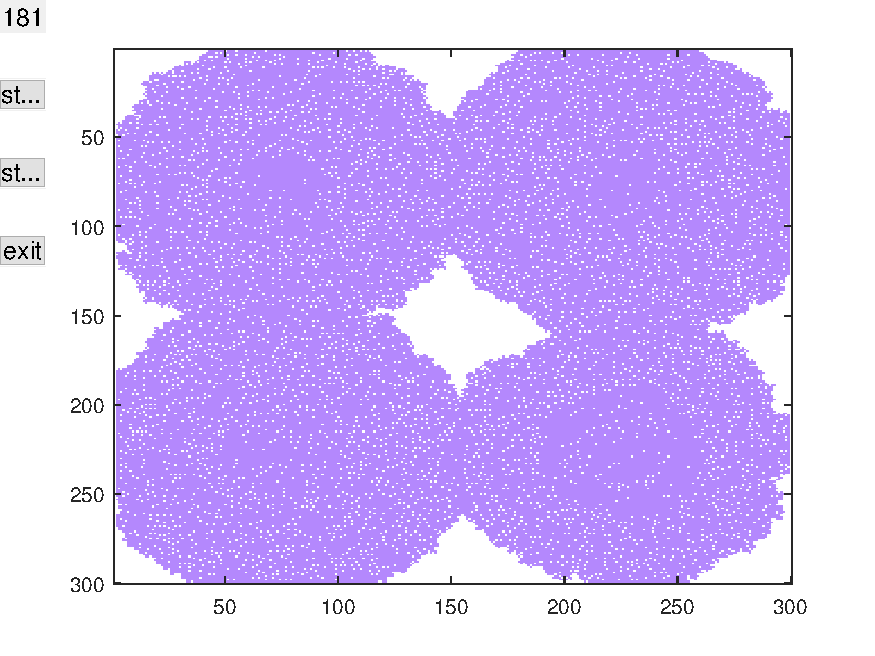
\includegraphics[height=10cm]{./T5Figure/K1N2/K1N2F.pdf}
	\caption{Algorithm schematic}
\end{figure}
\begin{figure}[H] 
	\centering 
	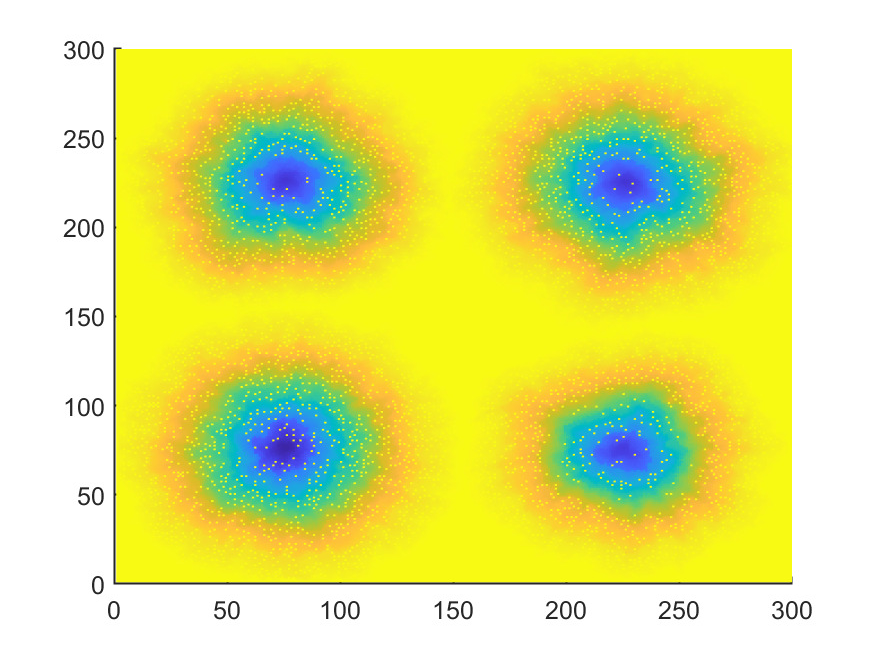
\includegraphics[height=10cm]{./T5Figure/K1N2/K1N2L.pdf}
	\caption{Algorithm schematic}
\end{figure}

\begin{figure}[H] 
	\centering 
	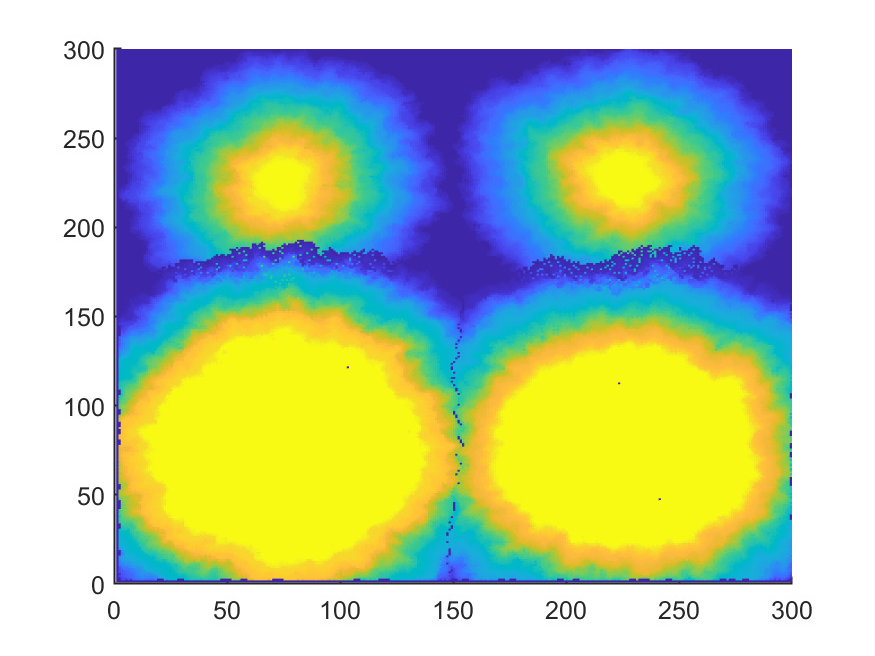
\includegraphics[height=10cm]{./T5Figure/K2N1/K2N1A.pdf}
	\caption{Algorithm schematic}
\end{figure}
\begin{figure}[H] 
	\centering 
	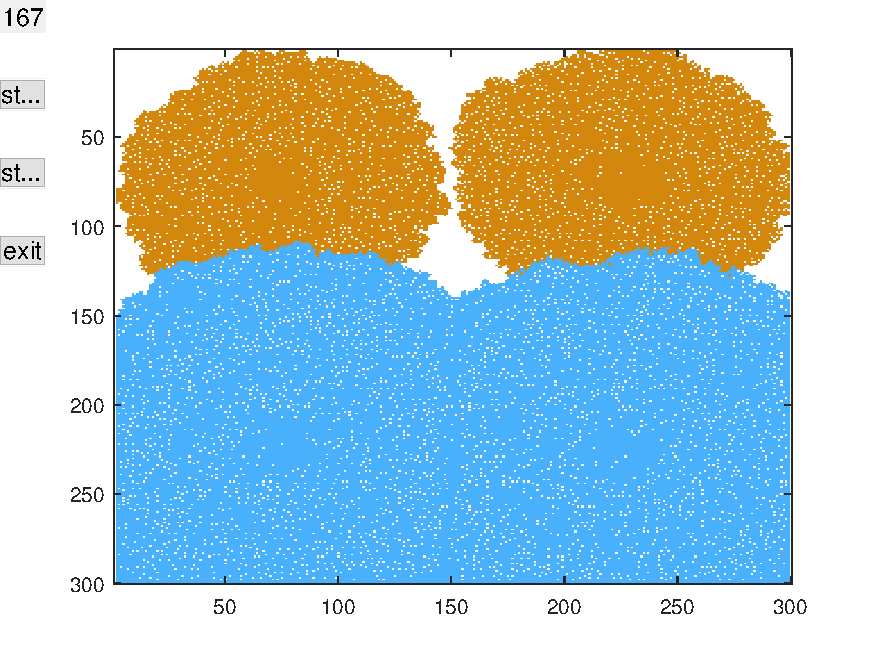
\includegraphics[height=10cm]{./T5Figure/K2N1/K2N1F.pdf}
	\caption{Algorithm schematic}
\end{figure}
\begin{figure}[H] 
	\centering 
	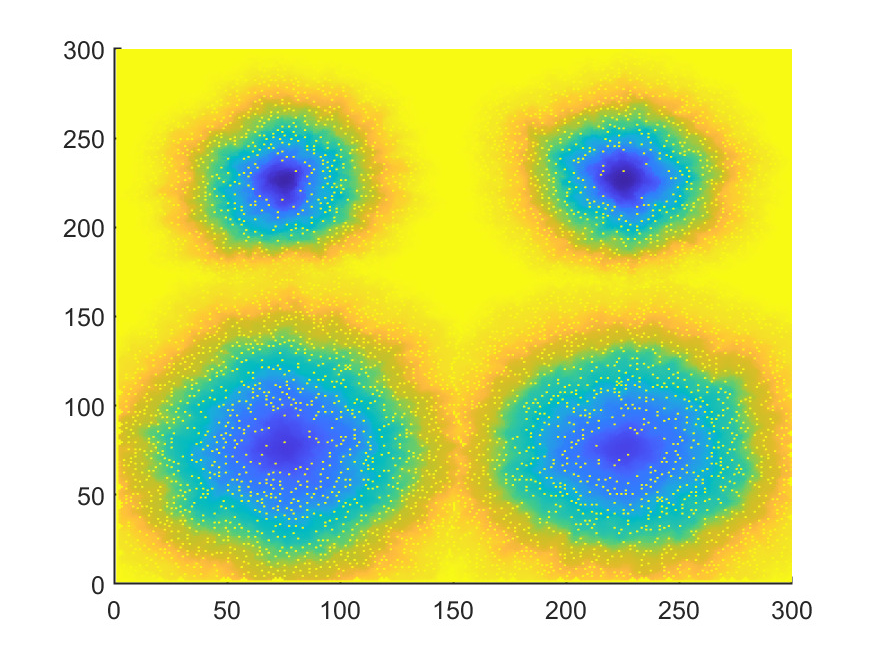
\includegraphics[height=10cm]{./T5Figure/K2N1/K2N1L.pdf}
	\caption{Algorithm schematic}
\end{figure}

\begin{figure}[H] 
	\centering 
	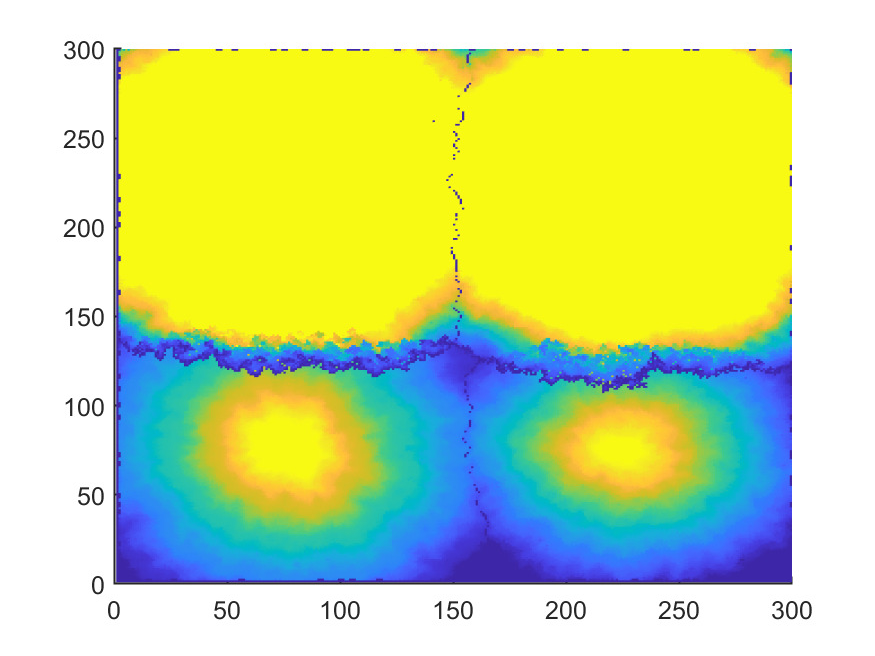
\includegraphics[height=10cm]{./T5Figure/K2N2/K2N2A.pdf}
	\caption{Algorithm schematic}
\end{figure}
\begin{figure}[H] 
	\centering 
	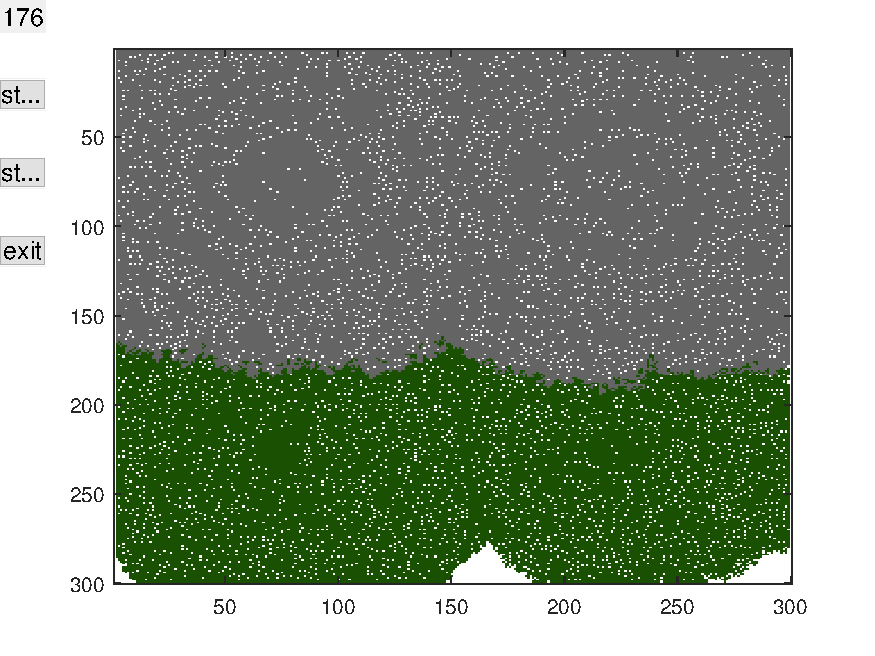
\includegraphics[height=10cm]{./T5Figure/K2N2/K2N2F.pdf}
	\caption{Algorithm schematic}
\end{figure}
\begin{figure}[H] 
	\centering 
	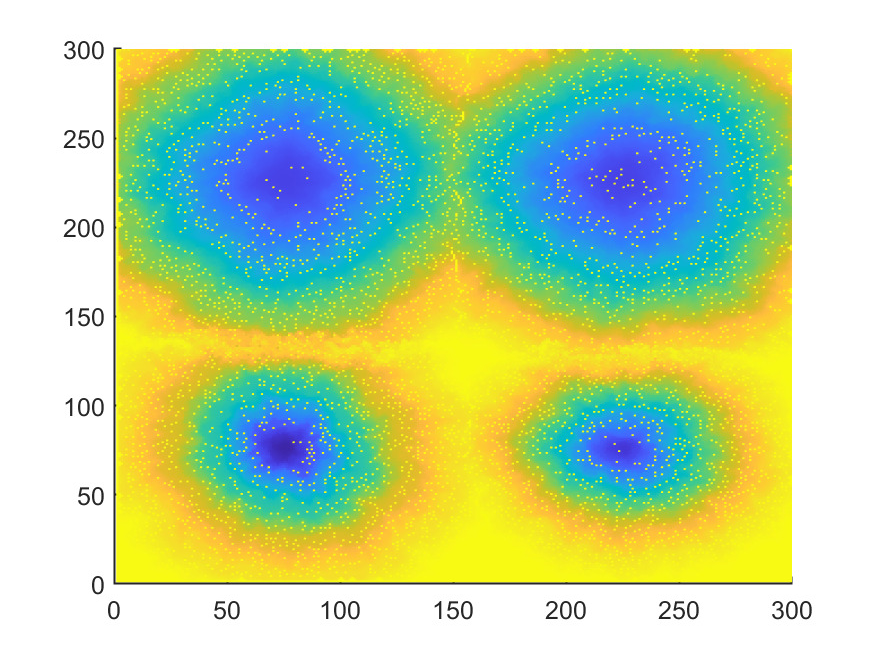
\includegraphics[height=10cm]{./T5Figure/K2N2/K2N2L.pdf}
	\caption{Algorithm schematic}
\end{figure}

\begin{figure}[H] 
	\centering 
	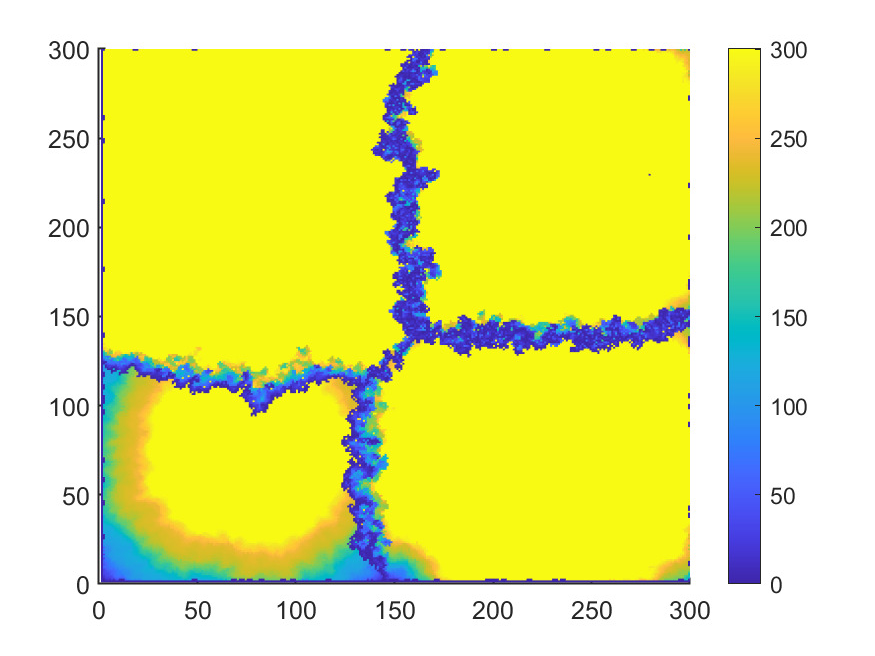
\includegraphics[height=10cm]{./T5Figure/K4N1/K4N1A.pdf}
	\caption{Algorithm schematic}
\end{figure}
\begin{figure}[H] 
	\centering 
	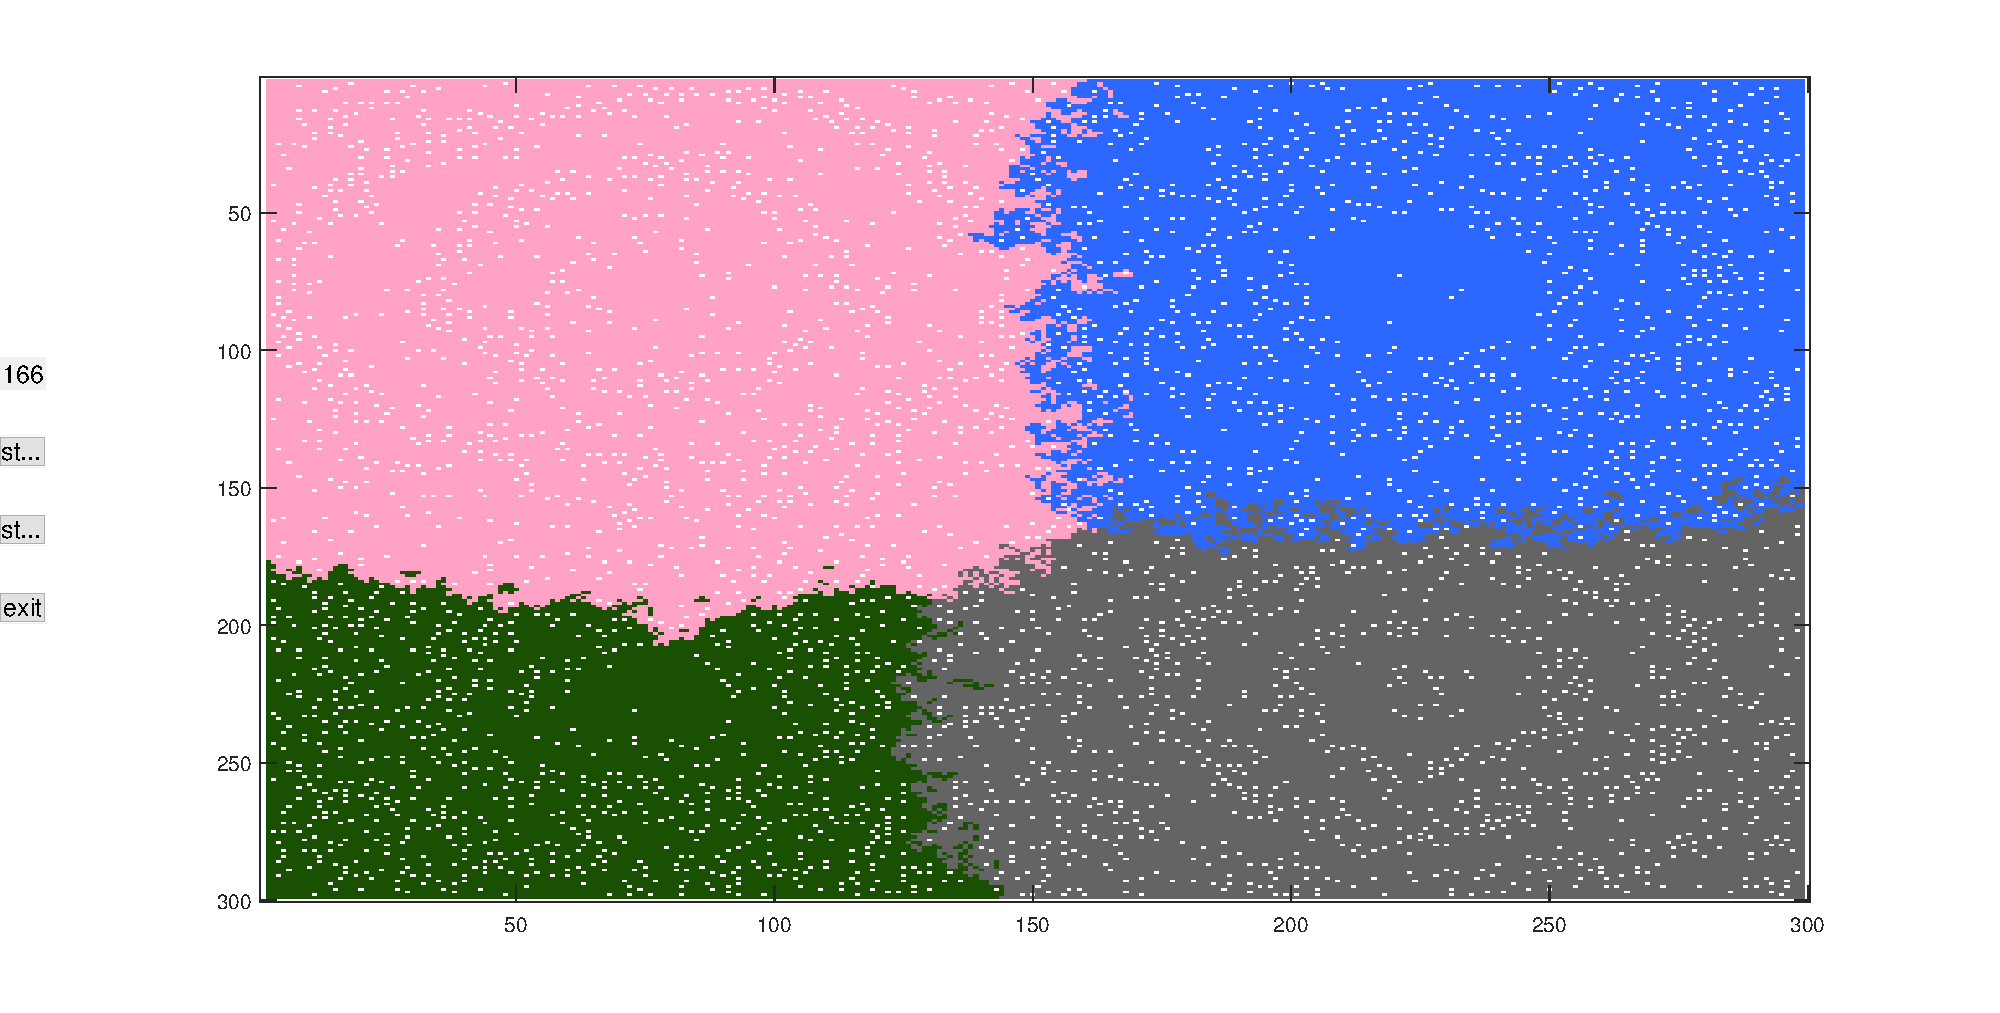
\includegraphics[height=10cm]{./T5Figure/K4N1/K4N1F.pdf}
	\caption{Algorithm schematic}
\end{figure}
\begin{figure}[H] 
	\centering 
	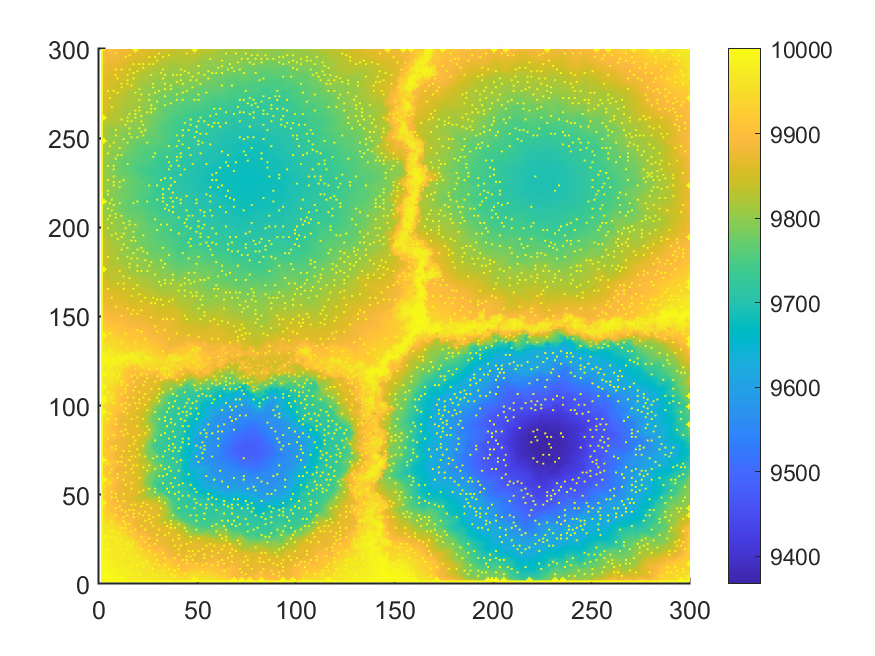
\includegraphics[height=10cm]{./T5Figure/K4N1/K4N1L.pdf}
	\caption{Algorithm schematic}
\end{figure}

\newpage
\section{Strength and Weakness}
\subsection{Strength}
\begin{itemize}
	\item A scientific and accurate simulation model is established by using \textbf{cellular automata} in MATLAB. \textbf{Excellent visualization} of fungal growth process makes the output of the model more intuitive, and also adds a lot of fun when solving the model.
	\item \textbf{Continuous problem discretization}: It is easy to update the model and consider more influence factors. At the same time, it enhances the robustness of the model and makes the model more stable.
	\item We simulate the change and influence of temperature and moisture in a very \textbf{large range}, including long-term and short-term simulation under eight different conditions (Boston/completely random environment/fixed value/five climate types).
\end{itemize} 
\subsection{Possible Improvements}
\begin{itemize}
	\item In our model, we only consider the competition relationship between fungi, but there are \textbf{other relationships} between them, such as cooperation.
	\item As the model becomes larger and larger, the \textbf{time} required to run a simulation code will become correspondingly longer. So when all the factors were taken into account, the computer is not fast enough to support the interaction of more than ten fungi on too many cells.
\end{itemize}
\section{Sensitivity Analysis}
\par In section 5.4, we have proved that our model is \textbf{sensitive to the rapid and drastic changes of temperature and moisture}. This is because different fungi have different optimal temperature and moisture. In our model, although the behavior pattern of each cell is complex, the overall behavior pattern of fungi is predictable according to some existing rules and our simulation results is exactlky consistent with these rules.
\par \textbf{Initial location} is also an important factor affecting the final results, so in the process of solving all the previous models, the initial position of fungi is fixed. Here we want to test whether the initial position of fungi will have a great impact on the final area occupied by it when there are multiple fungi exists.
\par The following Fig.\eqref{qwert} shows the results of the sensitivity analysis of the initial position. We fix the temperature and moisture and choose three different fungi (F5/F9/F12) for testing. Before each run of the cellular automata, we randomly generate initial positions for the three fungi and repeate the simulation for 50 times. Finally, we fit three curves for them using Matlab and because the slope of the three curves is close to 0, we can conclude that our model is \textbf{insensitive to the initial position of the fungus when the number of tests is large enough}.
\begin{figure}[H] 
	\centering 
	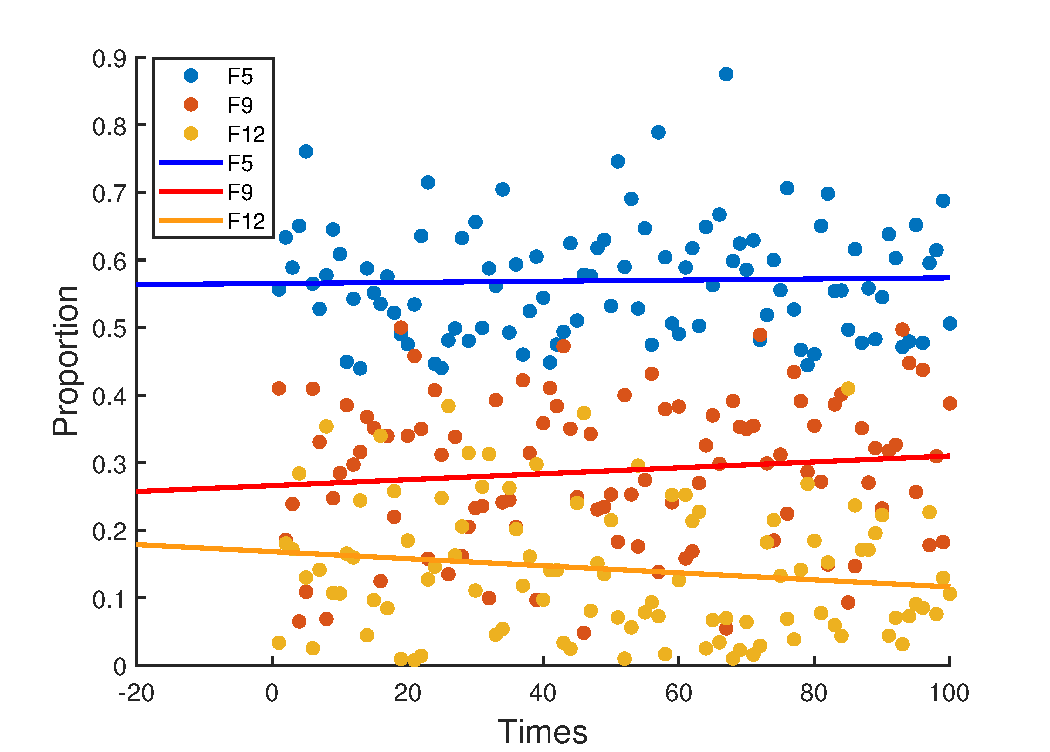
\includegraphics[height=8cm]{./picture/sensitivity.pdf}
	\caption{Algorithm schematic}
	\label{qwert}
\end{figure}

\newpage
\begin{appendices}
\section{Code Example}
\lstinputlisting[language=Matlab]{code/gene.m}

\end{appendices}
\end{document}


